
\begin{lead}

 システムの設計や解析,あるいはシステムの効率的な構成法の検討を行う場合には,前章で述べたインパルス応答のように,時間信号としてシステムを表現するだけでは不便である.そこで,$z$変換やフーリエ変換と呼ばれる変換法を用いて,信号やシステムを変換した形式で検討することが広く行われている.

 本章では,まず,\index{zへんかん@z変換}$z$変換という信号の変換法について説明する.

\end{lead}

%\vfill

%\begin{koumoku}
%システムの設計\\
%システムの解析\\
%$z$変換\\
%システムの伝達関数\\
%システムの周波数特性\\
%\end{koumoku}

%\clearpage


\chapter[$z$変換とシステムの伝達関数]{$z$変換と\\システムの伝達関数}

\label{chapter:40}

\section{$z$変換}

ここでは,$z$変換の定義,$z$変換の具体的な計算法,$z$変換の性質について,それぞれ説明する.

\subsection{$z$変換の定義}

離散時間信号$x(n)$の$z$変換$X(z)$は次式で定義される.
\begin{equation}
X(z)=\sum_{n=-\infty}^{\infty}x(n)z^{-n}
\label{eqn:eqn-3-01}
\end{equation}
%
ここで,$z$は一般に複素数値をとる複素変数である.

数列$x(n)$の$z$変換が$X(z)$であるとき,これらの関係を以下のように表現する.
\begin{equation}
x(n) \overset{z}{\leftrightarrow} X(z)
\end{equation}
\begin{equation}
Z[x(n)]=X(z)
\end{equation}

\subsection{インパルス$\delta(n)$の$z$変換}

具体的な$z$変換の計算例を示す.\index{いんぱるす@インパルス}インパルス$\delta(n)$の$z$変換は1である.すなわち,次式のように表現できる.
\begin{equation}
\delta(n) \overset{z}{\leftrightarrow} 1
\label{eqn:eqn-3-4}
\end{equation}

なぜ,このようになるかを以下に示す.
%
インパルスの定義は,
\begin{equation}
\delta(n)= \left \{
\begin{array}{ll}
1, & n=0 \\
0, & n\neq 0
\end{array}
\right .
\end{equation}
であるから,式(\ref{eqn:eqn-3-01})に$x(n)=\delta(n)$を代入すると,
\begin{equation}
Z[\delta(n)]=\sum_{n=-\infty}^{\infty}\delta(n)z^{-n}=\delta(0)z^{-0}=1
\label{eqn:eqn-3-1}
\end{equation}
となるので,式(\ref{eqn:eqn-3-1})が成立することがわかる\footnote{この$n_1\delta(n-n_0)$の$z$変換がわかると,$2\delta(n-3)$などの$z$変換の場合において,$n_1=2$,$n_0=3$とおくことで求めることができるようになる.
}.


類似の例として,$n_1\delta(n-n_0)$の$z$変換を求める.

\begin{eqnarray}
Z[n_1\delta(n-n_0)]&=&n_1\sum_{n=-\infty}^{\infty}\delta(n)z^{-n} \nonumber \\
 &=&n_1\delta(0)z^{-n_0} \nonumber \\
 &=&n_1z^{-n_0}
\label{eqn:eqn-3-6}
\end{eqnarray}\vskip.3\baselineskip

インパルスを用いて任意の信号$x(n)$を表現できることから,インパルスに対する$z$変換がわかれば,容易に$z$返還を求めることができるのである.

\subsection{$z$変換の性質}

ところで,$z$変換を行うにあたっては,以下に示すような$z$変換の性質を理解する必要がある.

\subsubsection{線形性}

任意の2つの信号$x_1(n)$,$x_2(n)$の$z$変換をそれぞれ$X_1(z)=Z[x_1(n)]$,$X_2(z)=Z[x_2(n)]$とすると,次式のような\index{せんけいせい@線形性}線形性の性質が成立する.

\begin{eqnarray}
Z[ax_1(n)+bx_2(n)]&=&Z[ax_1(n)]+Z[bx_2(n)] \nonumber \\
 &=&aZ[x_1(n)]+bZ[x_2(n)] \nonumber \\
 &=&aX_1(z)+bX_2(z)
\label{eqn:eqn-3-10}
\end{eqnarray}\vskip.3\baselineskip

\noindent ここで,$a$, $b$は任意の定数である.この性質から式(\ref{eqn:eqn-3-6})を導き出すことができる.


\subsubsection{時間シフト}

信号$x(n)$の$z$変換が$X(z)=Z[x(n)]$であるとき,次式のような\index{じかんしふと@時間シフト}時間シフトの関係が成り立つ.
\begin{equation}
x(n-k) \overset{z}{\leftrightarrow} X(z)z^{-k}, \hspace{1cm}(k:任意の整数)
\label{eqn:eqn-3-11}
\end{equation}

このことから,$x(n)$の$z$変換がわかれば,$n-k$なる時間シフトが発生する場合に$x(n)$の$z$変換に$z^{-k}$を掛ければ,$x(n-k)$の$z$変換が求められることがわかる.

\subsubsection{たたみ込み}

任意の2つの信号$x_1(n)$,$x_2(n)$の$z$変換をそれぞれ$X_1(z)=Z[x_1(n)]$,$X_2(z)=Z[x_2(n)]$とする.このとき,これらが\index{たたみこみ@たたみ込み}たたみ込みの関係にあるときは次式が成立する.
\begin{equation}
\sum_{k=-\infty}^{\infty}x_1(k)x_2(n-k) \overset{z}{\leftrightarrow} X_1(z)X_2(z)
\label{eqn:eqn-3-12}
\end{equation}

このように,たたみ込みの関係の場合における$z$変換は,それぞれの$z$変換を求めて掛け合わせればよい.

このような関係になることを証明する.

\begin{eqnarray}
Z[\sum_{k=-\infty}^{\infty}x_1(k)x_2(n-k)]&=&\sum_{n=-\infty}^{\infty}\sum_{k=-\infty}^{\infty}x_1(k)x_2(n-k)z^{-n} \nonumber \\
 &=&\sum_{n=-\infty}^{\infty}x_1(k)\sum_{k=-\infty}^{\infty}x_2(n-k)z^{-n} \nonumber \\
 & & (n-k=p と置き換える)\nonumber \\
 &=&\sum_{n=-\infty}^{\infty}x_1(k)\sum_{p=-\infty}^{\infty}x_2(p)z^{-p}z^{-k} \nonumber \\
 &=&\sum_{n=-\infty}^{\infty}x_1(k)X_2(z)z^{-k} \nonumber \\
 &=&X_2(z)\sum_{n=-\infty}^{\infty}x_1(k)z^{-k} \nonumber \\
 &=&X_2(z)X_1(z) \nonumber \\
 &=&X_1(z)X_2(z)
\label{eqn:eqn-3-13}
\end{eqnarray}\vskip.3\baselineskip

これらのような,$z$変換の性質である線形性,時間シフト,シフトの3つを理解すると,計算が非常に容易になる.

\section{システムの伝達関数}
\label{section:3-2}

第\ref{chapter:ch-2}章では,\index{いんぱるすおうとう@インパルス応答}インパルス応答が\index{せんけいときふへんしすてむ@線形時不変システム}線形時不変システムの情報をすべて持っていることを述べた.
ここでは,インパルス応答に代わる表現として,システムの伝達関数を定義する.
IIRシステムのように,インパルス応答では無限の表現が必要となるシステムに対しても,伝達関数は有限な表現を与え,表現がより簡潔になる.

\subsection{伝達関数の定義}

線形時不変システムにおいて,入力信号$x(n)$,インパルス応答$h(n)$と出力信号$y(n)$との間に,次式のような関係のたたみ込みが成り立つとする.
\begin{equation}
y(n)=\sum_{k=-\infty}^{\infty}h(k)x(n-k)
\end{equation}
この式を$z$変換すると,
\begin{equation}
Y(z)=H(z)X(z)
\label{eqn:eqn-3-14}
\end{equation}
と表現できる.ただし,$Y(z)=Z[y(n)]$,$H(z)=Z[h(n)]$,$X(z)=Z[x(n)]$である.

ここで,インパルス応答$h(n)$の$z$変換である$H(z)$を,システムの伝達関数(transfrt function)という.この伝達関数$H(z)$は,式(\ref{eqn:eqn-3-14})を用いると,
\begin{equation}
H(z)=\frac{Y(z)}{X(z)}
\label{eqn:eqn-3-15}
\end{equation}
とおくことができ,インパルス応答$h(n)$の$z$変換というだけでなく,入力信号$x(n)$の$z$変換である$X(z)$と,出力信号$y(n)$の$z$変換である$Y(z)$との比ということもできる.

\subsection{非再帰型システムの伝達関数}

\index{ひさいきがたしすてむ@非再帰型システム}非再帰型システムは\index{FIRしすてむ@FIRシステム}FIRシステムのことでもある.この非再帰型システムの伝達関数を求めるために,システムのインパルス応答を求めてから伝達関数を求める方法と,入出力信号をそれぞれ$z$変換してから伝達関数を求める方法との2つをそれぞれ比較する.

例として,次式のような3点平均を求めるシステムを考える.
\begin{equation}
y(n)=\frac{1}{3}(x(n)+x(n-1)+x(n-2))
\label{eqn:eqn-3-16}
\end{equation}

まず,システムのインパルス応答を求めてから伝達関数を求める方法によると,このシステムのインパルス応答$h(n)$は,
\begin{equation}
h(n)=\frac{1}{3}(\delta(n)+\delta(n-1)+\delta(n-2))
\end{equation}
であるから,伝達関数$H(z)$はこのインパルス応答$h(n)$を$z$変換すればよく,
\begin{equation}
H(z)=\frac{1}{3}(1+z^{-1}+z^{-2})
\end{equation}
が求められる.

次に,入出力信号をそれぞれ$z$変換してから伝達関数を求める方法によると,式(\ref{eqn:eqn-3-16})を$z$変換すると,

\begin{eqnarray}
Y(z)&=&\frac{1}{3}(X(z)+X(z)z^{-1}+X(z)z^{-2}) \nonumber \\
 &=&\frac{1}{3}(1+z^{-1}+z^{-2})X(z)
\end{eqnarray}\vskip.3\baselineskip

\noindent であるから,伝達関数$H(z)$は,
\begin{equation}
H(z)=\frac{Y(z)}{X(z)}=\frac{1}{3}(1+z^{-1}+z^{-2})
\label{eqn:eqn-3-19}
\end{equation}
が求められる.

これらのように,どちらのアプローチを用いても本質的には同じ結果が得られる.しかしながら,入出力信号をそれぞれ$z$変換してから伝達関数を求める方法のほうが簡便であるようだ.

\subsection{伝達関数の一般形}

非再帰型システムの伝達関数の一般形を考える.因果性を満たす非再帰型システムに対しては,
\begin{equation}
y(n)=\sum_{k=0}^{N-1}h(k)x(n-k), \hspace{5mm}(N: 正の整数)
\end{equation}
と表現され,たたみ込みの特殊な場合に相当する.伝達関数を求めると,

\begin{eqnarray}
Y(z)&=&\sum_{n=-\infty}^{-\infty}\sum_{k=0}^{N-1}h(k)x(n-k)z^{-n} \nonumber \\
 &=&\sum_{n=-\infty}^{-\infty}\sum_{k=0}^{N-1}h(k)x(n-k)z^{-(n-k)}z^{-k} \nonumber \\
 &=&\sum_{k=0}^{N-1}h(k)\sum_{n=-\infty}^{-\infty}x(n-k)z^{-(n-k)}z^{-k} \nonumber \\
 &=&\sum_{k=0}^{N-1}h(k)X(z)z^{-k} \nonumber \\
 &=&\sum_{k=0}^{N-1}[h(k)z^{-k}]X(z)
\end{eqnarray}\vskip.3\baselineskip

\noindent となるから,両辺を$X(z)$で割って,次式のように得ることができる.

\begin{equation}
H(z)=\frac{Y(z)}{X(z)}=\sum_{k=0}^{N-1}[h(k)z^{-k}]
\label{eqn:eqn-3-22}
\end{equation}
このように伝達関数は$z$多項式であり,この多項式の次数を伝達関数の次数(order)と呼ぶ.式(\ref{eqn:eqn-3-22})の場合であれば伝達関数の次数は$N-1$次であり,3点平均のシステムにおける伝達関数である式(\ref{eqn:eqn-3-19})の場合は伝達関数の次数は2次である.

\subsection{伝達関数の構成}

ところで,次式に示されるような伝達関数を持つシステムは,図\ref{fig:zu-3-4}に示すような構成により実現される.

\begin{equation}
H(z)=\frac{Y(z)}{X(z)}=\sum_{k=0}^{N-1}[h(k)z^{-k}]
\label{eqn:eqn-3-22-1}
\end{equation}

\begin{figure}[H]
\begin{center}
\begin{minipage}{.4\textwidth}
\begin{center}
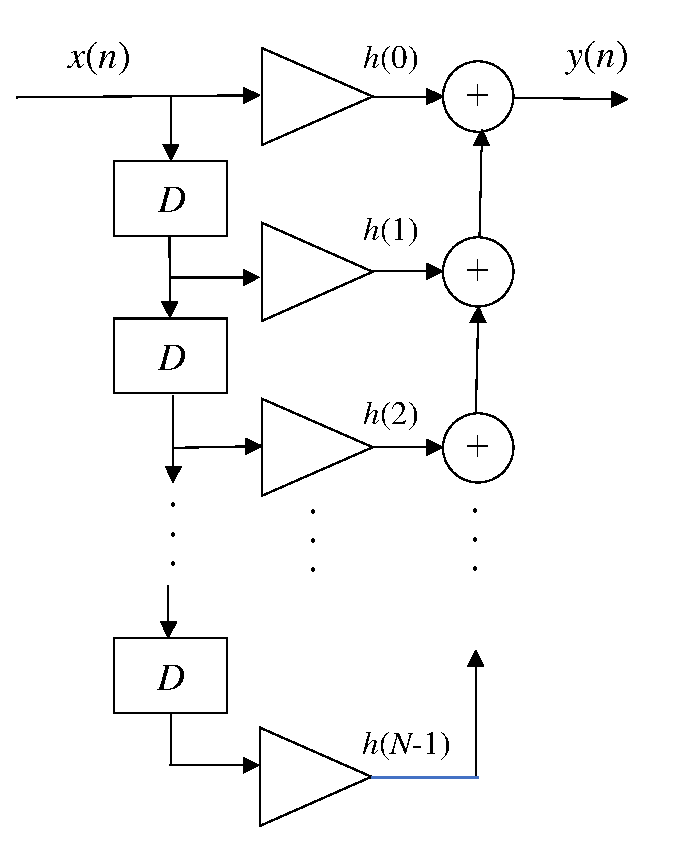
\includegraphics[width=.95\textwidth]{fig/zu-2-12.eps}

(a)たたみ込みの表現
\end{center}
\end{minipage}
\begin{minipage}{.4\textwidth}
\begin{center}
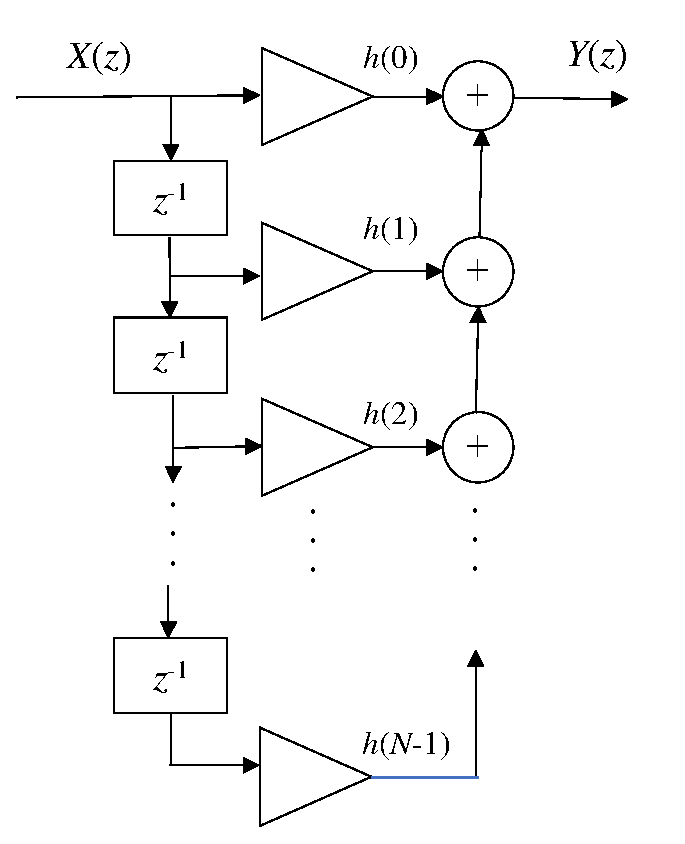
\includegraphics[width=.95\textwidth]{fig/zu-3-4.eps}

(b) $z$領域の表現
\end{center}
\end{minipage}
\end{center}\vskip.5\baselineskip
\caption{非再帰型システムの構成}
\label{fig:zu-3-4}
\end{figure}



この構成は,先述の図\ref{fig:zu4-2-12}に示すような構成に対応する.ここで,$z^{-1}$については,図中の``$D$''と同様に信号をシフトする\index{ちえんき@遅延器}遅延器を表している.この遅延器の入出力の関係は$y(n)=x(n-1)$で表されるので,その$z$変換は次式のように表される.
\begin{equation}
Y(z)=z^{-1}X(z)
\label{eqn:eqn-3-23}
\end{equation}

\section{再帰的システムの伝達関数}

ここでは,フィードバックを持つ再帰型システムの伝達関数について説明する.
IIRシステムはフィードバックを持つ再帰的システムとして実現されるので,伝達関数を求めることと,伝達関数の極の概念について示す.

\subsection{\index{さいきてきしすてむ@再帰的システム}再帰的システムの導出法}

フィードバックを持つシステムの例として,以下の式について伝達関数を導出する.
\begin{equation}
y(n)=x(n)+by(n-1)
\label{eqn:eqn-3-24}
\end{equation}
ここで$b$は定数である\footnote{このように右辺に出力$y(n)$を持つシステム表現を,定係数差分方程式と呼ぶ.}.

この場合のシステムの伝達関数を求めるために,両辺を$z$変換すると,
\begin{equation}
Y(z)=X(z)+bY(z)z^{-1}
\end{equation}
となり,左辺に$Y(z)$の項で,右辺に$X(z)$の項でまとめると,
\begin{equation}
Y(z)(1-bz^{-1})=X(z)
\end{equation}
であるから,伝達関数$H(z)$は次式のようになる.
\begin{equation}
H(z)=\frac{Y(z)}{X(z)}=\frac{1}{1-bz^{-1}}
\end{equation}

この伝達関数について,改めてインパルス応答から求めてみる.式(\ref{eqn:eqn-3-24})のインパルス応答は,
\begin{equation}
y(n)\sum_{k=0}^{\infty}b^x(n-k)
\end{equation}
であることから,この$z$変換は,
\begin{equation}
Y(z)=\sum_{k=0}^{\infty}b^kz^{-k}X(z)
\end{equation}
であるから,伝達関数$H(z)$は\footnote{等比級数について,初項$a$で公比$r$($|r|<1$)の場合,

$\displaystyle a(1+r+r^2+r^3+\cdots) = a\sum_{k=0}^{\infty}r = \frac{a}{1-r}$

である.ここでは,初項が1で公比が$br^{-1}$となる.
},
\begin{equation}
H(z) = \frac{Y(z)}{X(z)} %\nonumber \\
  = \sum_{k=0}^{\infty}b^kz^{-k} %\\
  = \frac{1}{1-bz^{-1}}
\end{equation}
となる.

このように,再帰的システムの伝達関数は,解くためのプロセスに関係なく同じ結果が得られることがわかる.


\subsection{伝達関数の一般形}

定係数差分方程式の一般形は,次式のように表される.
\begin{equation}
y(n)=\sum_{k=0}^{M}a_kx(n-k)-\sum_{k=1}^{N}b_ky(n-k)
\end{equation}
この両辺を$z$変換すると,
\begin{equation}
Y(z)=\sum_{k=0}^{M}a_kz^{-k}X(z)-\sum_{k=1}^{N}b_kz[^{-1}Y(z)
\end{equation}
となるので,求める伝達関数は次式のようになる.
\begin{equation}
H(z)=\frac{Y(z)}{X(z)}=\frac{\displaystyle \sum_{k=0}^{M}a_kz^{-k}}{1+ \displaystyle \sum_{k=1}^{N}b_kz{^{-1}}} \label{eqn:eqn-3-28}
\end{equation}

この式が,再帰型システムの伝達関数の一般形である.ここで,整数$M$と$N$のうち大きい方を,\index{でんたつかんすうのじすう@伝達関数の次数}伝達関数の次数という.

この再帰的システムの伝達関数におけるポイントは以下の通りに集約される.
\begin{itemize}
\item 伝達関数の分子は式(\ref{eqn:eqn-3-28})の入力$x(n-k)$の係数から決まる.
\item 伝達関数の分母は式(\ref{eqn:eqn-3-28})の出力$y(n-k)$の係数に対応し,図\ref{fig:figure-5-2}におけるフィードバック項を決定する.
\item すべての$b_k$が0のとき,非再帰型システムに帰着する.
\item 伝達関数の分母の係数$b_k$は,式(\ref{eqn:eqn-3-28})の出力$y(n-k)$の係数($-b_k$)と逆符号である.(移項の際に符号が反転する)
\end{itemize}

また,再帰型システムの構成を図\ref{fig:figure-5-2}に示す.

\begin{figure}[H]
\begin{center}
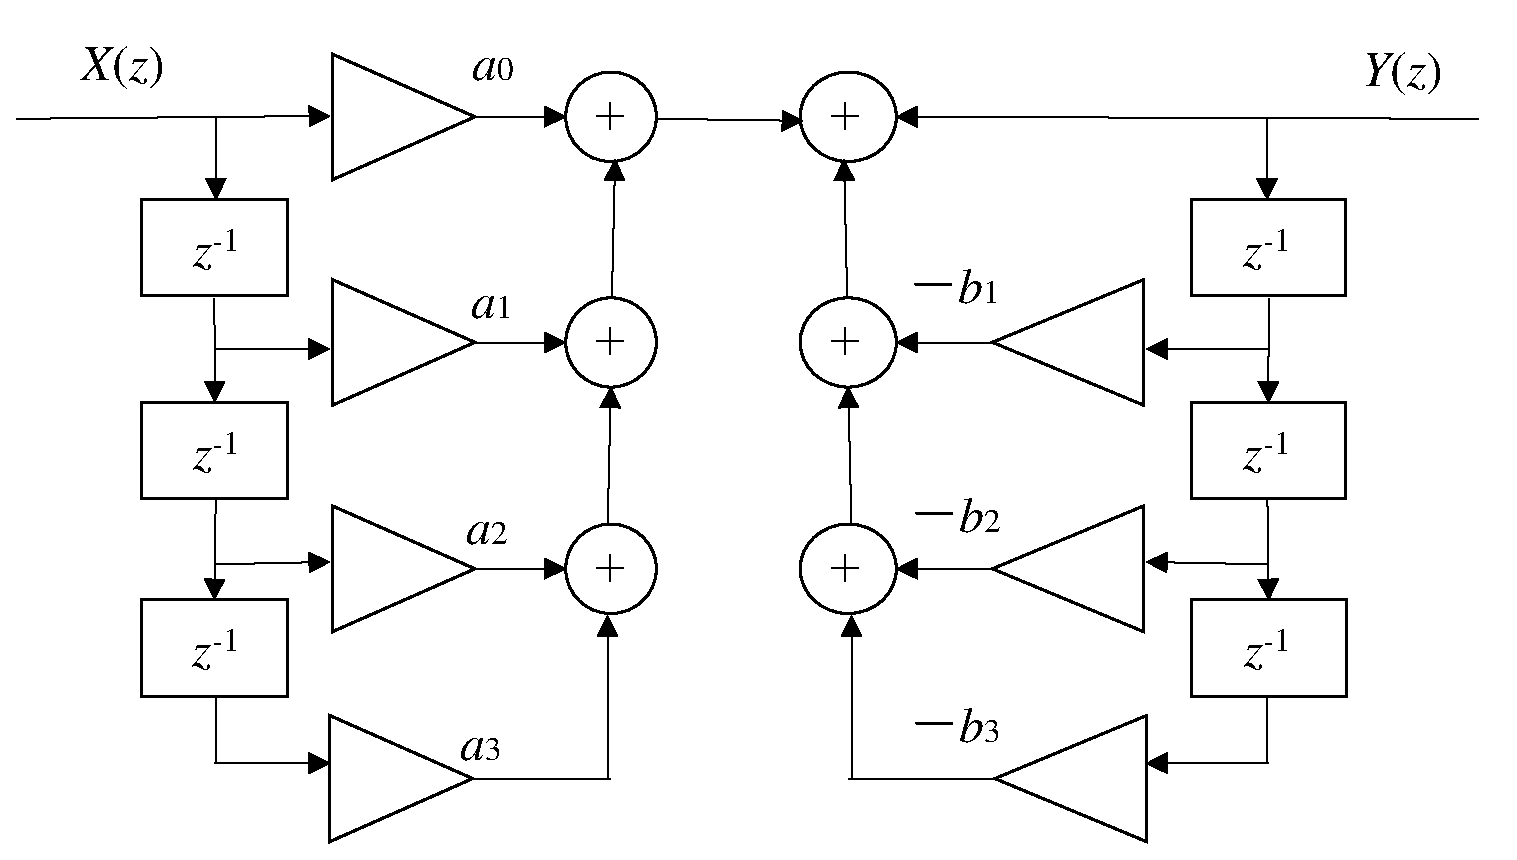
\includegraphics[width=9cm]{fig/figure-5-2.eps}
\end{center}
\caption{再帰型システムの構成}
\label{fig:figure-5-2}
\end{figure}

\newpage

\subsection{伝達関数の零点と極}

伝達関数の特徴を調べる際には,伝達関数の\index{ぜろてん@零点}零点と\index{きょく@極}極を用いる.
%
ここで,次式のような一般的な伝達関数を考える.
\begin{equation}
H(z)=\frac{Y(z)}{X(z)}=\frac{\displaystyle \sum_{k=0}^{M}a_kz^{-k}}{1+ \displaystyle \sum_{k=1}^{N}b_kz{^{-1}}} \label{eqn:eqn-3-30}
\end{equation}

このように伝達関数は$z$多項式の比で与えられる.このため,多項式は,多項式の次数と等しい数の根を有する.この根のうち,$H(z)=0$となる$z$の根を伝達関数の零点(zero)と呼び,$H(z)=\infty$となる$z$の根を伝達関数の極(pole)と呼ぶ.零点は\index{ぶんしたこうしき@分子多項式}分子多項式の根に相当し,極は\index{ぶんぼたこうしき@分母多項式}分母多項式の根に相当する.

具体例として,\index{3てんへいきん@3点平均}3点平均の伝達関数の場合を考える.この場合の伝達関数は,
\begin{equation}
H(z)=\frac{1}{3}(1+z^{-1}+z^{-2})
\end{equation}
である.この零点と極を求めるために,次式のように書き換える.

\begin{eqnarray}
H(z)&=&\frac{1}{3z^2}(z^2+z+1) \nonumber \\
 &=&\frac{\displaystyle \left (z-\frac{-1+j\sqrt{3}}{2} \right ) \left ( z-\frac{-1-j\sqrt{3}}{2} \right ) }{3z^2} \\
 &=&a\frac{(z-z_{00})(z-z_{01})}{(z-z_{p0})(z-z_{p1})}
\end{eqnarray}\vskip.3\baselineskip

\noindent ここで,$z_{00}$, $z_{01}$は零点であり,$z_{p0}$, $z_{p1}$は極である.
%
この式から,零点$Z_{00}$, $Z_{01}$は,次式のようになる.
\begin{equation}
z_{00}=\frac{-1+j\sqrt{3}}{2}
\end{equation}
\begin{equation}
z_{01}=\frac{-1-j\sqrt{3}}{2}
\end{equation}
また,極$z_{p0}$, $z_{p1}$は次式のように重根である.
\begin{equation}
z_{p0}=z_{p1}=0
\end{equation}

この例でもわかるように,非再帰型システムの伝達関数の極は,すべて原点の存在する.ここで説明した零点と極を用いた伝達関数の特徴に関する議論は次章にて述べる.

\newpage

\section*{演習問題}

\subsection*{問題\ref{chapter:40}.1}

以下の信号の$z$変換を求めよ.

(1) $x(n)=\delta(n+2)+3\delta(n)-2\delta(n-1)$

(2) $x(n)=u(n)+2u(n-1)$

(3) $x(n)=-b^nu(-n-1)$

(4) $x(n)=\sin(\omega n)u(n)$

\subsection*{問題\ref{chapter:40}.2}

信号$x(n)$の$z$変換を$X(z)$とする.以下の信号の$z$変換を$X(z)$を用いて表せ.

(1) $y(n)=ax(n)+bx(n-d)$

(2) $y(n)=(-1)^nx(n)$


